\documentclass[12pt,a4paper,portrait]{article}
%\setcounter{secnumdepth}{0}
\usepackage{gensymb}
\usepackage{pdflscape}
\usepackage{amsmath}
\usepackage{amssymb}
\usepackage{enumitem}
\usepackage{graphicx}
\usepackage{subcaption}
\usepackage{multirow}
\usepackage{sansmath}
\usepackage{pst-eucl}
\usepackage{multicol}
\usepackage{csquotes}
% Coding
\usepackage{listings}
\setlength{\parindent}{0pt}
\usepackage[obeyspaces]{url}
% Better inline directory listings
\usepackage{xcolor}
\definecolor{light-gray}{gray}{0.95}
\newcommand{\code}[1]{\colorbox{light-gray}{\texttt{#1}}}
\usepackage{adjustbox}
\usepackage[UKenglish]{isodate}
\usepackage[UKenglish]{babel}
\usepackage{float}
\usepackage[T1]{fontenc}
\usepackage{setspace}
\usepackage{sectsty}
\usepackage{longtable}
\newenvironment{tightcenter}{%
	\setlength\topsep{0pt}
	\setlength\parskip{0pt}
	\begin{center}
	}{%
	\end{center}
}
\captionsetup{width=\textwidth}
\usepackage{mbenotes} % to print table notes!
\usepackage{alphalph} % For extended counters!
% usage: \tabnotemark[3]\cmsp\tabnotemark[4]
\usepackage[colorlinks=true,linkcolor=blue,urlcolor=black,bookmarksopen=true]{hyperref}
\sectionfont{%			            % Change font of \section command
	\usefont{OT1}{phv}{b}{n}%		% bch-b-n: CharterBT-Bold font
	\sectionrule{0pt}{0pt}{-5pt}{3pt}}
\subsectionfont{
	\usefont{OT1}{phv}{b}{n}}
\newcommand{\MyName}[1]{ % Name
	\usefont{OT1}{phv}{b}{n} \begin{center}of {\LARGE  #1}\end{center}
	\par \normalsize \normalfont}
\makeatletter
\newcommand\FirstWord[1]{\@firstword#1 \@nil}%
\newcommand\@firstword{}%
\newcommand\@removecomma{}%
\def\@firstword#1 #2\@nil{\@removecomma#1,\@nil}%
\def\@removecomma#1,#2\@nil{#1}
\makeatother

\newcommand{\MyTitle}[1]{ % Name
	\Huge \usefont{OT1}{phv}{b}{n} \begin{center}#1\end{center}
	\par \normalsize \normalfont}
\newcommand{\NewPart}[1]{\section*{\uppercase{#1}}}
\newcommand{\NewSubPart}[1]{\subsection*{\hspace{0.2cm}#1}}
\renewcommand{\baselinestretch}{1.05}
\usepackage[margin=0.2cm]{geometry}
\date{}
\title{Pendulum on a cart on an inclined plane}
\author{Brenton Horne}

\begin{document}
	\maketitle
	\begin{figure}[H]
		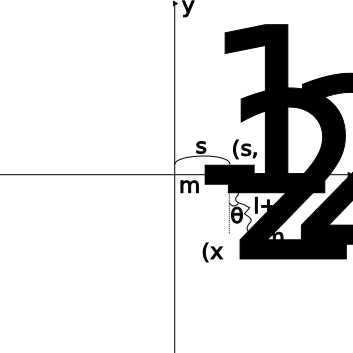
\includegraphics[width=300px]{Elastic pendulum on a cart.png}
		\caption{Diagram of problem.}\label{fig1}
	\end{figure}
	
	Here we have a cart whose centre of mass is at $(s, 0)$ and a pendulum attached to its horizontal centre bottom. To simplify calculations, we will assume the height of the cart is 0, but adding a constant height to the cart will not change the equations of motion. Hence the kinetic energy for the cart is $\dfrac{m_1}{2}\dot{s}^2$. Next, we will calculate the coordinates, velocity and kinetic energy of the pendulum
	
	\begin{align*}
		x_2 &= s + (l+z)\sin{\theta} \\
		\dot{x}_2 &= \dot{s} + \dot{z}\sin{\theta} + (l+z)\dot{\theta}\cos{\theta}\\
		y_2 &= -(l+z)\cos{\theta} \\
		\dot{y}_2 &= -\dot{z}\cos{\theta} + (l+z)\dot{\theta}\sin{\theta} \\
		v_2^2 &= \dot{x}_2^2 + \dot{y}_2^2 \\
		&= (\dot{s} + \dot{z}\sin{\theta} + (l+z)\dot{\theta}\cos{\theta})^2 + (-\dot{z}\cos{\theta} + (l+z)\dot{\theta}\sin{\theta})^2 \\
		&= \dot{s}^2 + \dot{z}^2 \sin^2{\theta} + (l+z)^2\dot{\theta}^2\cos^2{\theta} + 2\dot{s}\dot{z}\sin{\theta} + 2\dot{s}\dot{\theta}(l+z)\cos{\theta} + 2\dot{z}\dot{\theta}(l+z)\sin{\theta}\cos{\theta} + \dot{z}^2\cos^2{\theta} \\
		&+ (l+z)^2\dot{\theta}^2\sin^2{\theta} - 2\dot{z}\dot{\theta}(l+z)\cos{\theta}\sin{\theta}\\
		&= \dot{s}^2 + \dot{z}^2 + (l+z)^2\dot{\theta}^2 + 2\dot{s}(\dot{z}\sin{\theta} + \dot{\theta}(l+z)\cos{\theta})\\
		T_p &= \dfrac{m_2}{2} \left(\dot{s}^2 + \dot{z}^2 + (l+z)^2\dot{\theta}^2 + 2\dot{s}(\dot{z}\sin{\theta} + \dot{\theta}(l+z)\cos{\theta})\right).
	\end{align*}
	
	Hence the total kinetic energy of the system is
	
	\begin{align*}
		T &= T_c + T_p \\
		&= \dfrac{m_1}{2}\dot{s}^2 + \dfrac{m_2}{2} \left(\dot{s}^2 + \dot{z}^2 + (l+z)^2\dot{\theta}^2 + 2\dot{s}(\dot{z}\sin{\theta} + \dot{\theta}(l+z)\cos{\theta})\right) \\
		&= \dfrac{m_1+m_2}{2} \dot{s}^2 + \dfrac{m_2}{2}\left(\dot{z}^2 + (l+z)^2\dot{\theta}^2 + 2\dot{s}(\dot{z}\sin{\theta} + \dot{\theta}(l+z)\cos{\theta})\right).
	\end{align*}
	
	As for the potential energy, it comes in two forms --- gravitational and spring. 
	
	\begin{align*}
		V &= m_2 g y_2 + \dfrac{kz^2}{2}\\
		&= -m_2g(l+z)\cos{\theta} + \dfrac{kz^2}{2}.
	\end{align*}
	
	Hence the Lagrangian is
	
	\begin{align*}
		\mathcal{L} &= T - V \\
		&= \dfrac{m_1+m_2}{2} \dot{s}^2 + \dfrac{m_2}{2}\left(\dot{z}^2 + (l+z)^2\dot{\theta}^2 + 2\dot{s}(\dot{z}\sin{\theta} + \dot{\theta}(l+z)\cos{\theta})+2g(l+z)\cos{\theta}\right) - \dfrac{kz^2}{2}.
	\end{align*}
\end{document}
	